\subsection{Hierarchical Methods}
If clusters were ``allowed'' to have sub clusters, then we would then 
automatically obtain a hierarchical clustering method \citep{tan05}. This 
clustering method simply groups objects into a tree of clusters. The root node 
of the tree contains all clusters, with each node (cluster) in the tree the 
union of its children.

There are two branches of hierarchical clustering, agglomerative and divisive. 
The only difference between the two is the direction in which clustering 
happens \citep{tan05}.

The agglomerative algorithm utilises a bottom-up (merging) strategy, whereas 
the divisive algorithm utilises a top-down (separating) strategy \citep{tan05}. 
Figure \ref{fig:hierarchicalDefinition} shows the two forms of hierarchical 
clustering side by side. 

\begin{figure}[H]
  \centering
  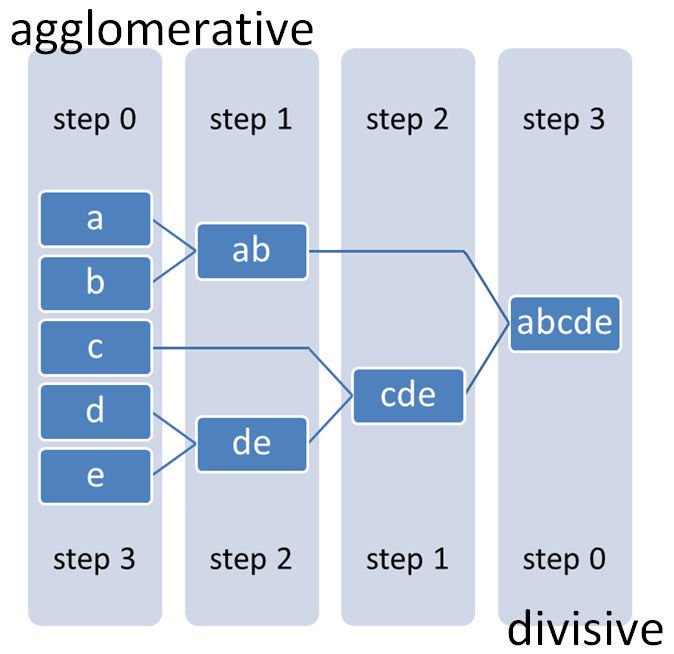
\includegraphics[width=0.7\linewidth]{chapter3/clustering/hierarchical.png}
  \label{fig:hierarchicalDefinition}
  \caption
   {Two main methods of clustering hierarchically.}
\end{figure}

The agglomerative method initially places each object into a cluster of its own, 
and the clusters are then merged according to some criterion, such as Euclidean 
distance \citep{tan05}. 

The process of merging clusters to form larger embedded clusters continues 
until one cluster is formed. The last cluster could be thought of as the `root 
cluster' \citep{han06}.

In contrast, the divisive method will place all objects into one initial cluster. 
The algorithm will then split this cluster into child clusters based upon a 
criterion \citep{tan05}. 

The criterion could be anything, but as with the agglomerative method the 
Euclidean distance between the closest neighbouring objects in the cluster is 
a popular criterion. The splitting process continues until each new cluster 
only contains a single object \citep{han06}.

One of the key elements to hierarchical clustering is the computation of the 
proximity between two clusters --- proximity matrix --- \citep{tan05}. It is 
this definition that will change with each variation of the algorithms. 

There are three methods to calculate the proximity between two clusters
\citep{tan05}. These are outlined below:

\begin{itemize} 
  \item \textbf{Single Link} (MIN) defines the cluster proximity as the 
        proximity between the closest two objects within two different 
        clusters. 
        \begin{figure}[H]
          \centering
          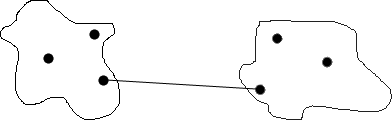
\includegraphics[width=0.60\linewidth]{chapter3/clustering/min.png}
        \end{figure}

  \item \textbf{Complete Link} (MAX) defines the cluster proximity as the 
        proximity between two farthest objects within two different clusters.
        \begin{figure}[H]
          \centering
          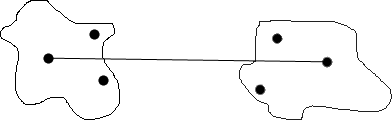
\includegraphics[width=0.60\linewidth]{chapter3/clustering/max.png}
        \end{figure}

  \item \textbf{Group Average} defines the cluster proximity as the average 
        pairwise proximities of all pairs of objects from two different 
        clusters.
        \begin{figure}[H]
          \centering
          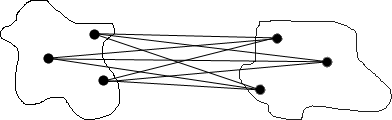
\includegraphics[width=0.60\linewidth]{chapter3/clustering/group_average.png}
        \end{figure}
\end{itemize}


\subsubsection{Agglomerative}
The agglomerative algorithm is a bottom-up strategy, and hence all objects are 
placed into their own cluster \citep{tan05}. The algorithm will then merge the 
two closest pair of clusters, and will continue doing this in order to create 
larger and larger clusters. 

The end point of the algorithm is reached when all of the objects are in a 
single cluster. Each specific implementation of the agglomerative algorithm 
is the same, differing only in the definition of inter-cluster similarity 
\citep{tan05}.

\paragraph*{Agglomerative Formal Algorithm}
\subparagraph*{Input:}
\begin{itemize}
  \item {\bf D} - the data set of {\em n} objects
\end{itemize}

\subparagraph*{Output:}
\begin{itemize}
  \item A set of clusters
\end{itemize}

\subparagraph*{Method:}
\begin{enumerate}
  \item Compute the proximity matrix (may not be required);
  \item {\bf repeat}
  \item \begin{list}{$\square$}{\leftmargin=1em \itemindent=0em}
          Merge the closest two clusters;
        \end{list}
  \item \begin{list}{$\square$}{\leftmargin=1em \itemindent=0em}
          Update the proximity matrix for both the new and original clusters;
        \end{list}
  \item {\bf until one} cluster remains.
\end{enumerate}

Agglomerative algorithms produce an ordering of the objects 
\citep{iosHierarchical}, which can be advantageous for data display, where the 
ordering of the data might be important. 

Agglomerative algorithms also have a tenancy to produce smaller clusters, which
can be helpful for knowledge discovery \citep{iosHierarchical}.

The agglomerative algorithm is unable to perform an adjustment (undo) once the 
merge process has been completed. This means that if a chosen merge turns out 
to be unsound, the method is unable to backtrack, and an entire re-run of the 
algorithm would be required \citep{tan05}. 

\subsubsection{Divisive}
The divisive algorithm is a top-down strategy \citep{han06}. All the objects 
are initially placed into one cluster. At each step, a cluster will be split, 
and this will be repeated until each cluster has exactly one cluster 
\citep{tan05}. 

The main decision of this algorithm is to correctly decide which cluster to 
split up at each stage, and how exactly do to the splitting. As with the 
agglomerative algorithm, the specific implementation of the divisive algorithm 
is the same, differing only in the definition of inter-cluster similarity 
\citep{tan05}.

\paragraph*{Divisive Formal Algorithm}
\subparagraph*{Input:}
\begin{itemize}
  \item {\bf D} - the data set of {\em n} objects
\end{itemize}

\subparagraph*{Output:}
\begin{itemize}
  \item A set of clusters
\end{itemize}

\subparagraph*{Method:}
\begin{enumerate}
  \item 1.  Place all objects into one cluster;
  \item {\bf repeat}
  \item \begin{list}{$\square$}{\leftmargin=1em \itemindent=0em}
          Find the object which has the highest average dissimilarity in 
          comparison to the other objects. Place this object into a new 
          cluster, C;
        \end{list}
  \item \begin{list}{$\square$}{\leftmargin=1em \itemindent=0em}
          {\bf repeat}
        \end{list}   
  \item \begin{list}{$\square$}{\leftmargin=1em \itemindent=0em}
          \begin{list}{$\square$}{\leftmargin=1em \itemindent=0em}
            For each object X not in C, compute the distance;
          \end{list}  
        \end{list}        
  \item \begin{list}{$\square$}{\leftmargin=1em \itemindent=0em}
          \begin{list}{$\square$}{\leftmargin=1em \itemindent=0em}
            If the distance $>$ 0, then merge the object X to C
          \end{list}  
        \end{list}   
  \item \begin{list}{$\square$}{\leftmargin=1em \itemindent=0em}
          {\bf until} all the distances calculated are negative;
        \end{list} 
  \item \begin{list}{$\square$}{\leftmargin=1em \itemindent=0em}
          Choose the cluster with the largest dissimilarity between any of its 
          two objects, and divide this cluster;
        \end{list} 
  \item {\bf until all} clusters contain one object;
\end{enumerate}

As with the agglomerative algorithm, the divisive algorithm produces an ordering
of the objects, which can be advantageous for data display. Smaller clusters 
are generally generated, which can be helpful for knowledge discovery 
\citep{iosHierarchical}.

As with the agglomerative algorithm, the divisive algorithm is unable to 
perform an adjustments (undo) once the split process has been completed. An 
entire re-run of the algorithm would be required, if a chosen split turned out
to be unsound \citep{tan05}.
